\problemname{\problemyamlname}

\begin{wrapfigure}{r}{5.5cm}
	\centering
	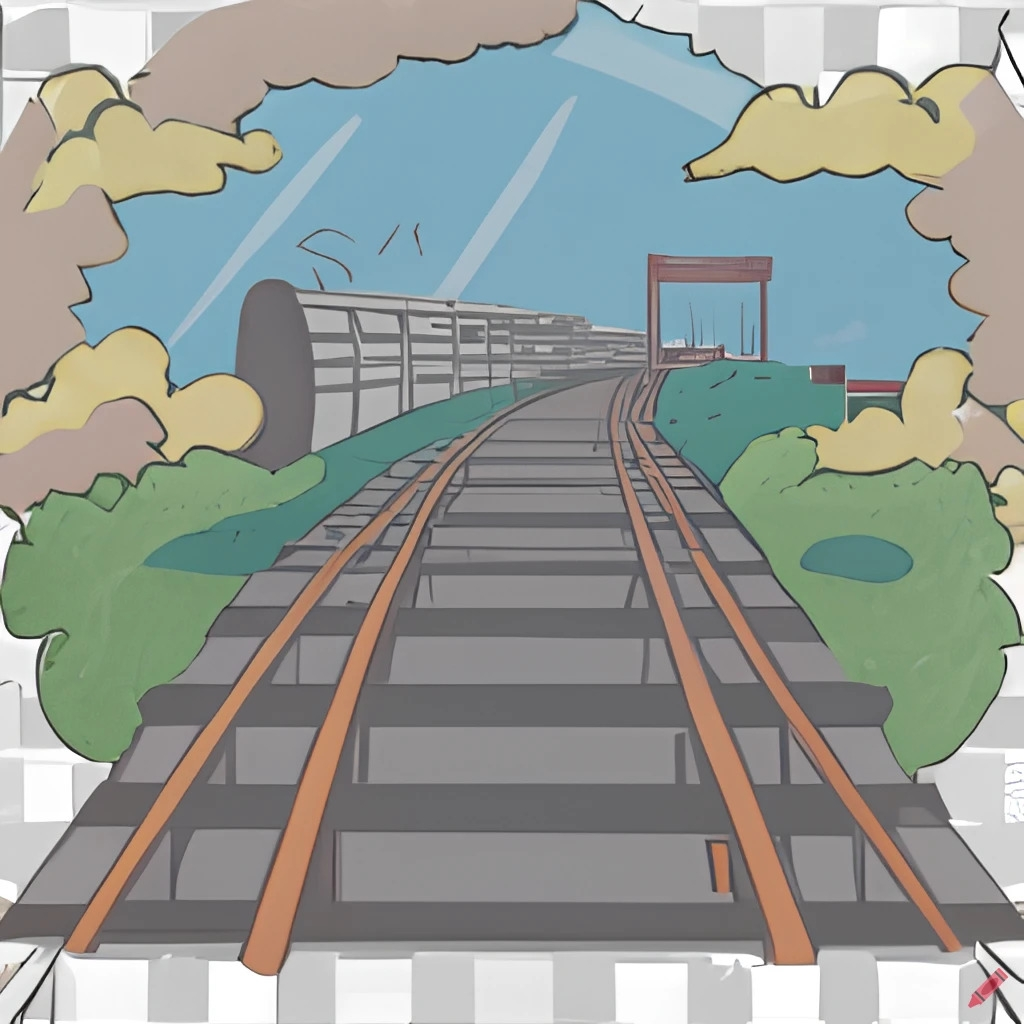
\includegraphics[width=5.5cm]{railway.jpg}
\end{wrapfigure}

In the context of the \emph{Comfortable Circuit} campaign, Bertand Karwa and his Securail team are temporarily reassigned to managing the safety of multiple Belgian train lines.
They receive a list of the lines to take between two stations, and they must pass at least once over each line so as to show to the train passengers their presence and, thus, to reassure them.

They would like to optimize their path so as to take each train line exactly once, independently of the direction in which they're taking it.
However, they are unsure of the feasibility of this task.
Help them to determine if it's possible \textbf{starting at a given station} to follow a path to return at that \textbf{same station} and passing by each train line \textbf{once and only once}.

\begin{Input}
	The input consists of:
	\begin{itemize}
		\item One line with an integer $n$ ($3 \le n \le 10^3$), the number of paths that Mr. Karwa and his team must take.
		\item One line with the name of a station, where Mr. Karwa and his team must depart from.
		\item $n$ lines containing a path to take, that is two string separated by a space ``\verb|station1 station2|'' to say that they must take the line from ``\verb|station1|'' to ``\verb|station2|'' or from ``\verb|station2|'' to ``\verb|station1|'' (but not both).
	\end{itemize}
	The names of the stations are given as a lowercase alphabetic letter.
	A train line between two station will only be given once and acts as a bidirectional line.
\end{Input}

\begin{Output}
	If it's possible for Mr. Karwa and his team to visit each train line exactly once, show ``\verb|impossible|'', otherwise show ``\verb|ok|''.
\end{Output}
